\chapter{Ý tưởng giải thuật, các bài toán cốt lõi}
\setlength{\epigraphwidth}{0.5\textwidth}

\section{Visual Studio và Windows Form}
\textbf{Visual Studio} hay Microsoft Visual Studio là một môi trường phát triển tích hợp (IDE) từ Microsoft. Visual Studio còn được gọi là ``Trình soạn thảo mã nhiều người sử dụng nhất thế giới'', được dùng để lập trình C++ và C\# là chính. Nó được sử dụng để phát triển chương trình máy tính cho Microsoft Windows, cũng như các trang web, các ứng dụng web và các dịch vụ web. Visual Studio sử dụng nền tảng phát triển phần mềm của Microsoft như Windows API, Windows Forms, Windows Presentation Foundation, Windows Store và Microsoft Silverlight.

\textbf{Windows form} hay còn gọi là \textbf{Winform} là thuật ngữ mô tả một ứng dụng được viết trên .NET FrameWork và có giao diện đồ hoạ.

Để hiểu sâu hơn thì Windows Form là một thư viện lớp đồ họa, mã nguồn mở và hoàn toàn miễn phí. Từ năm 2003 thì windows form được xem là một phần của microsoft. Phần mềm này sẽ cung cấp nền tảng để viết những lập trình phong phú dành cho máy tính bàn, laptop, máy tính bảng,$\dots$ được coi như một sự thay thế cho thư viện lớp nền tảng Microsoft Foundation của C++.

Tuy nhiên đến năm 2014 thì Windows Form chính thức bị Microsoft khai tử. Windows Form có tuổi thọ khá lâu đời, chính vì thế nên chúng bị khai tử. Nhưng ở Việt Nam thì chúng vẫn được tồn tại và phát triển. Lý do là vì những ưu điểm mà chúng mang lại. Những lập trình viên C\# ở đời đầu cũng đều được học và sử dụng về Windows Form. Bởi vì:

\begin{itemize}
	\item Giao diện có thể kéo thả dễ học và sử dụng.
	\item Gắn các event cho các button chỉ cần double click. Hỗ trợ nhiều event như click, hover,$\dots$
	\item Viết code trực quan hơn: Có thể lấy text từ textbox và show dữ liệu bằng messagebox, kết nối grid bằng SQL.
\end{itemize}

Bên cạnh những ưu điểm của Windows Form thì chúng cũng có nhiều nhược điểm chưa được khắc phục sau đây:

\begin{itemize}
	\item Phần mềm chỉ có thể chạy trên nền tảng Windows Form.
	\item Windows Form chỉ phù hợp cho ứng dụng trên desktop (ứng dụng quản lý thông tin và tương tác trực tiếp với người dùng).
	\item Đồ họa không cao nên giao diện sẽ thiếu đi tính trực quan, không thân thiện đối với người dùng.
\end{itemize}

\begin{figure}[!h]
	\centering
	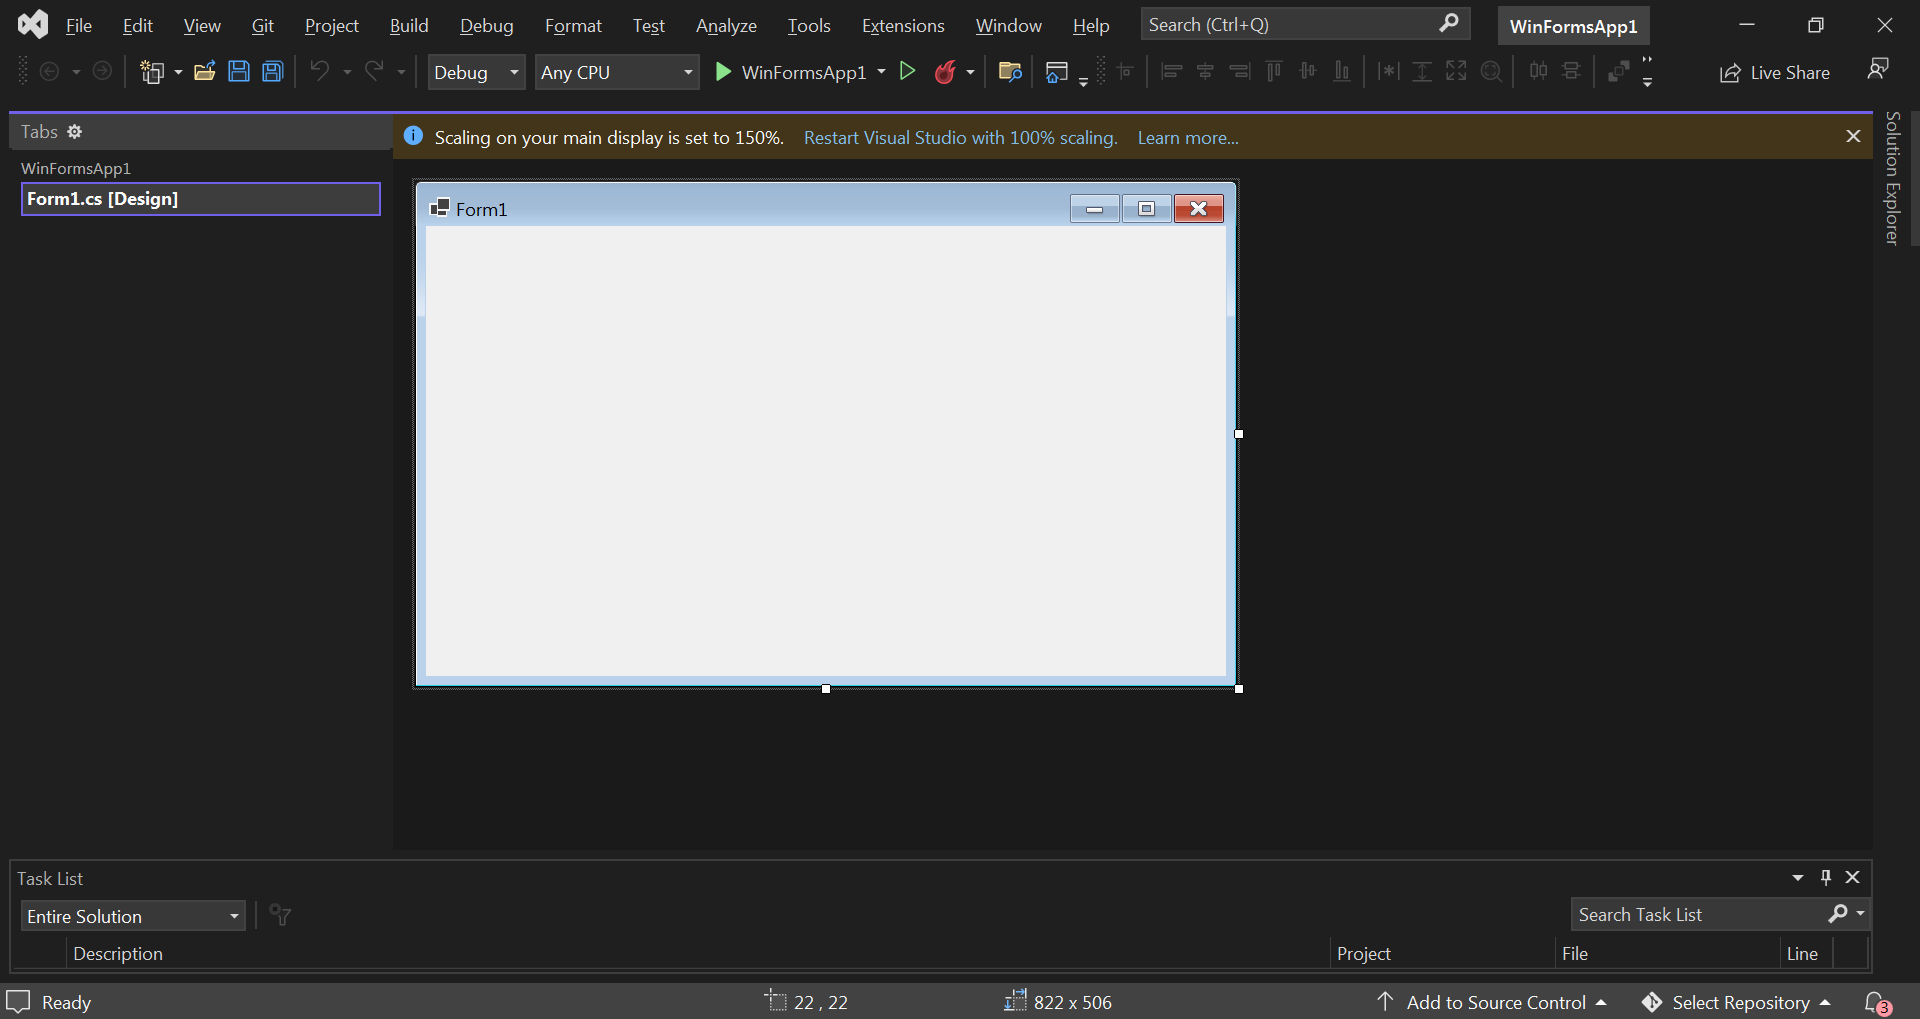
\includegraphics[scale=.42]{image/vs.png}
	\caption{\textit{Môi trường làm việc của project Windows Form trên Visual Studio}} 
\end{figure}

\section{Giao diện đồ hoạ (Graphical User Interface - GUI)}
Giao diện đồ họa hay giao diện người dùng trong tiếng Anh gọi tắt là \textit{GUI (Graphical User Interface)} là một thuật ngữ trong ngành công nghiệp máy tính. Đó là một cách giao tiếp với máy tính hay các thiết bị điện tử bằng hình ảnh và chữ viết thay vì chỉ là các dòng lệnh đơn thuần. GUI được sử dụng phổ biến trong máy tính, các thiết bị cầm tay, các thiết bị đa phương tiện, hoặc các linh kiện điện tử trong văn phòng, nhà ở,... Trong bài tiểu luận này game Caro sẽ được chạy trên giao diện đồ hoạ.

\begin{figure}[h!]
	\centering
	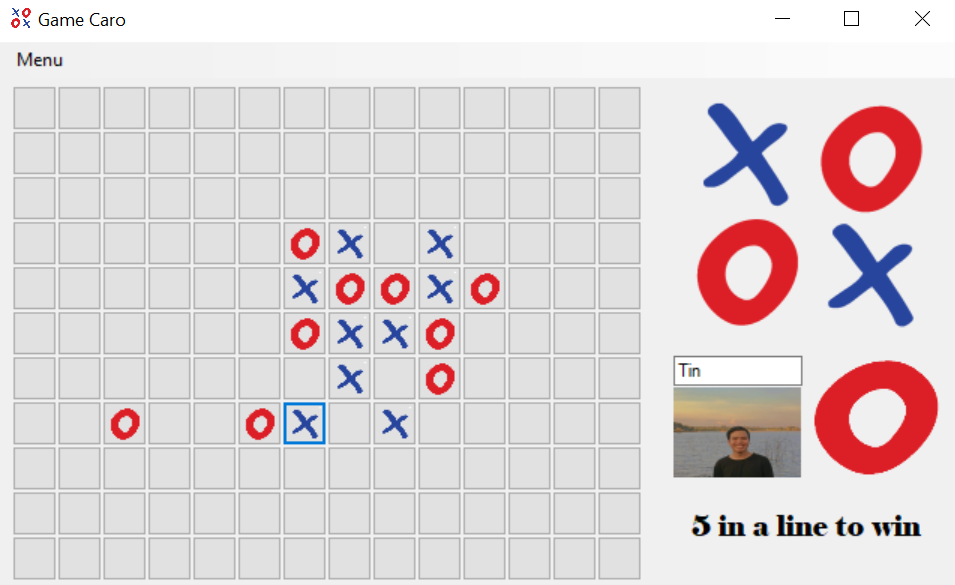
\includegraphics[scale=.90]{image/GUI.png}
	\caption{\textit{Trò chơi Caro trên giao diện đồ hoạ (Graphical User Interface - GUI)}} 
\end{figure}

\section{Tổng quan về một project, trong Winform}

\textbf{Project} (dự án) là cấp độ quản lý mã nguồn quan trọng nhất của C\#. Mỗi project sau khi biên dịch sẽ tạo ra một chương trình. Mỗi project mặc định đều chứa:
\newpage
\begin{itemize}
	\item \textbf{Các file mã nguồn:} là các file văn bản có phần mở rộng .cs (viết tắt của C sharp).
	\item \textbf{Các file cấu hình:} là file xml có phần mở rộng .config
	\item \textbf{Các thư viện được tham chiếu tới (References):} là danh sách các file thư viện chuẩn của .NET framework, hoặc thư viện từ các hãng thứ ba, hoặc chính các project khác, chứa các class được sử dụng bởi các class trong project này.
	\item \textbf{Các thuộc tính (Properties):} bao gồm nhiều các loại thông tin khác nhau quyết định những tính chất quan trọng của project, như phiên bản của .NET framework được sử dụng, loại chương trình mà dự án này sẽ được dịch thành, các tài nguyên được sử dụng trong project, cấu hình của ứng dụng,$\dots$Visual Studio cung cấp giao diện đồ hoạ để có thể dễ dàng quản lý các thông tin này. Giao diện này mở ra khi click đúp vào mục Properties của project.
\end{itemize}

\begin{figure}[h!]
	\centering
	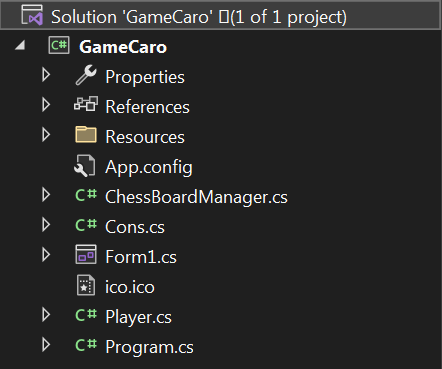
\includegraphics[scale=.99]{image/solution.png}
	\caption{\textit{Solution và Project trong C\#}} 
\end{figure}

Tất cả các thành phần của một project đều đặt chung trong một thư mục cùng tên với project.

\textbf{Solution} (giải pháp) là cấp độ quản lý mã nguồn cao nhất trong C\# cho phép quản lý tập trung nhiều project. Mỗi solution trong C\# có thể chứa nhiều project. Nếu solution không chứa project nào, nó gọi là Empty Solution. Tại mỗi thời điểm Visual Studio chỉ có thể mở một solution. 

Trên giao diện Visual Studio, solution và các project của nó được hiển thị trong một cửa sổ riêng gọi là Solution Explorer. Cửa sổ này hiển thị tất cả các thành phần trong dự án C\# theo cấu trúc cây, với solution làm gốc, các project là các nhánh trực tiếp xuất phát từ gốc này.

Ngoài ra để tiện lợi trong việc quản lý các project thành viên, solution cho phép tạo thêm các thư mục, gọi là Solution Folder, trong đó lại có thể chứa có project khác. Cấu trúc quản lý này cho phép quản lý một số lượng lớn project một cách dễ dàng. Các project trong cùng một solution thường có quan hệ nhất định với nhau.

\section{Cấu trúc file/thư mục của C\# project}

Nếu ở giai đoạn tạo project chúng ta đánh dấu lựa chọn ``Create directory for solution'', Visual Studio sẽ tạo ra một thư mục có tên được xác định trong mục ``Solution name''. Mỗi project được tạo ra sẽ đặt trong một thư mục con của thư mục solution và có cùng tên với project. Tất cả file của một project sẽ nằm trong thư mục này. 

Toàn bộ cấu hình của solution được lưu trong một file có phần mở rộng \textbf{.sln} nằm trong thư mục chứa solution. Thông tin cấu hình của dự án được lưu trong file có tên trùng với tên dự án và phần mở rộng \textbf{.csproj}.

\begin{figure}[h!]
	\centering
	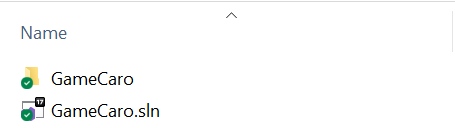
\includegraphics[scale=.99]{image/dic01.png}
	\caption{\textit{Thư mục Solution}} 
\end{figure}

\begin{figure}[h!]
	\centering
	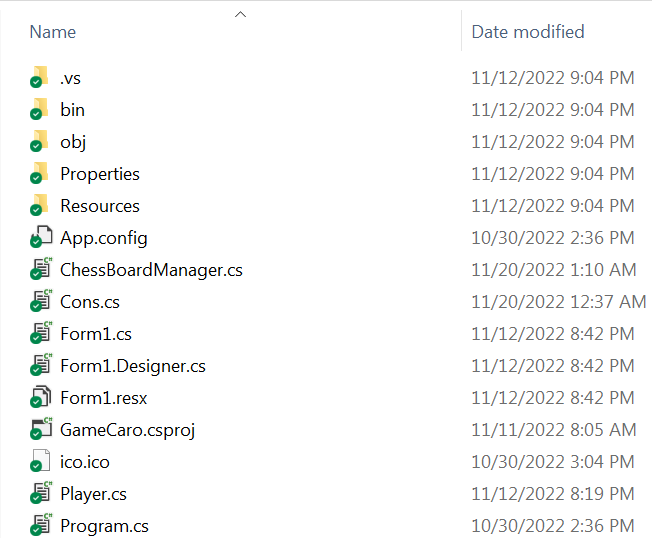
\includegraphics[scale=.99]{image/dic02.png}
	\caption{\textit{Thư mục Project}} 
\end{figure}

Sau khi biên dịch project thành công, trong thư mục của nó sẽ xuất hiện một thư mục con có tên là \textit{bin}. Thư mục này không xuất hiện trong cấu trúc dự án hiển thị ở Solution Explorer.

Nếu biên dịch ở chế độ debug, trong thư mục bin sẽ xuất hiện thư mục con Debug. File chương trình sau khi biên dịch (ở chế độ debug) xong sẽ xuất hiện trong thư mục này.

Nếu chạy chương trình ở chế độ debug (phím F5), thư mục Debug này sẽ trở thành thư mục hiện hành của chương trình đang chạy thử. Tất cả các file cấu hình và file tài nguyên (nếu có) cũng sẽ được tự động copy vào thư mục này.

\begin{figure}[h!]
	\centering
	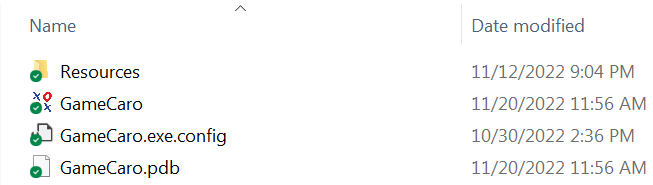
\includegraphics[scale=.99]{image/dic03.png}
	\caption{\textit{Thư mục bin}} 
\end{figure}

Như vậy, nếu bạn muốn tìm file chạy của chương trình sau khi biên dịch, hãy mở theo đường dẫn \textbf{\{tên đường dẫn\}$\backslash$\{tên project\}$\backslash$bin$\backslash$\{Debug\}}.

\section{Một số control trong Winform}
Trong phần này tác sẽ sẽ giới thiệu một số control trong C\# sử dụng trong dự án
\begin{description}
	\item [Panel]: Cho phép chứa đựng các điều khiển khác như: Button, RadioButton, Checkbox
	\item [PictureBox]: Cho phép hiển thị hình ảnh dạng bitmap, metafile, icon, JPEG, GIF.          
	\item [TextBox]: để nhập dữ liệu đầu vào, ngoài ra còn có thể dùng để xuất dữ liệu. Các ô tài khoản mật khẩu trên mạng xã hội, các ô nhập thông tin trong phần mềm, các ô lưu tên cho highscore khi chơi game, chúng ta có thể thấy textbox ở khắp mọi ứng dụng hiện nay.
	\item [MenuStrip]: là một điều khiển cho phép lập trình viên xây dựng hệ thống Menu trên Form. 
	\item [Label]: hiển thị nội dung, chữ.
	\item [Button]: là một thành phần tương tác cho phép người dùng giao tiếp với một ứng dụng. Lớp Button (Nút) kế thừa trực tiếp từ lớp ButtonBase. Có thể nhấp vào Button bằng cách sử dụng chuột, phím ENTER hoặc phím cách nếu Button đã được đặt tiêu điểm.
\end{description}
\section{Tạo bàn cờ}\label{sec:create-table}
Một bàn cờ thực chất là một ma trận mà mỗi ô là một Button (nút bấm). Ma trận này được khởi tạo như sau \;\texttt{Matrix = new List<List<Button>{}>} Các Button này có các điều chỉnh kích thước và toạ độ trên Form. Ở mỗi vòng lặp để xác định được vị trí cần tạo của Button mới ta cần một biến \texttt{oldButton} để lưu vị trí của Button trước đó. Và để tiện trong việc tạo ra ván game mới khi sử dụng chương trình, trước khi khởi tạo bàn cờ phương thức \texttt{DrawChessBoard()} sẽ thực hiện xoá hết các Control trên Panel bằng lệnh \texttt{ChessBoard.Controls.Clear()}.
\renewcommand{\lstlistingname}{Đoạn mã}% Listing -> Đoạn mã

\begin{lstlisting}[language={[Sharp]C}, caption = Phương thức \texttt{DrawChessBoard()}]
	public void DrawChessBoard()
	{
		ChessBoard.Controls.Clear();
		Matrix = new List<List<Button>>();
		Button oldButton = new Button() { Width = 0, Height = 0, Location = new Point(0, 0) };
		for (int i = 0; i < Cons.CHESS_BOARD_HEIGHT; i++)
		{
			Matrix.Add(new List<Button>());
			for (int j = 0; j < Cons.CHESS_BOARD_WIDTH; j++)
			{
				Button btn = new Button()
				{
					Width = Cons.CHESS_WIDTH,
					Height = Cons.CHESS_HEIGHT,
					Location = new Point(oldButton.Location.X + oldButton.Width, oldButton.Location.Y),
					BackgroundImageLayout = ImageLayout.Stretch,
					Tag = i.ToString()
				};

				btn.Click += btn_Click ;

				ChessBoard.Controls.Add(btn);

				Matrix[i].Add(btn);

				oldButton = btn;
			}
			oldButton.Location = new Point(0, oldButton.Location.Y + Cons.CHESS_HEIGHT);
			oldButton.Width = 0;
			oldButton.Height = 0;
		}
	}
\end{lstlisting}
Khi các người chơi thực hiện thao tác click vào các Button trên bàn cờ thì dòng 21 ở Đoạn mã sẽ thực hiện phương thức \texttt{btn\_Click()} thực hiện việc đổi hình ảnh nền của Button sang hình ảnh hiển thị quân cờ của người chơi hiện tại. Đồng thời gọi các phương thức \texttt{Mark()} thực hiện đổi người chơi và kí hiệu quân cờ của người chơi sau đó phương thức \texttt{ChangePlayer()} được gọi để chỉnh các thông tin người chơi vừa được đổi. Cuối cùng phương thức \texttt{btn\_Click()} gọi hàm \texttt{isEndgame()} để kiểm tra xem lần chơi cuối cùng đã kết thúc game chưa.
\begin{lstlisting}[language={[Sharp]C},label={code:btn_Click}, caption = Phương thức \texttt{btn\_Click()}]
	void btn_Click(object sender, EventArgs e)
	{
		Button btn = sender as Button;

		if (btn.BackgroundImage != null)
			return;
		
		Mark(btn);
		
		ChangePlayer();

		if (isEndGame(btn))
		{
			EndGame();
		}   
	}
\end{lstlisting}
\section{Xử lý đổi người chơi}
Trong hàm khởi tạo của class \texttt{ChessBoardManager} ta sẽ tạo ra một List có kiểu \texttt{Player}, lớp \texttt{Player} này sẽ chứa các thuộc tính liên quan đến thông tin người chơi. Lý do tạo List mà không tạo ra luôn hai người chơi cố định là để dễ dàng mở rộng chương trình sau này nếu muốn nhiều người chơi cùng lúc. Ta tạo thêm một biến \texttt{CurrentPlayer} kiểu \texttt{int} được gán giá trị là 0, dùng để lưu lượt của người chơi ở đây 0 tức là đang đến lượt người đầu tiên (vị trí 0 trong List). Và cũng nghĩa là chương trình mặc định cho người đầu chơi đầu tiên chơi List chơi trước.

Việc đổi người chơi sẽ được thực thi khi thực hiện việc click vào các Button trên Panel bàn cờ. Khi đó ta sẽ thực hiện hai phương thức là \texttt{Mark()} và \texttt{ChangePlayer()} trong phương thức \texttt{btn\_Click()} \ref{code:btn_Click}.

\begin{lstlisting}[language={[Sharp]C},label={code:btn_Click}, caption = Phương thức \texttt{btn\_Click()}]
	private void Mark(Button btn)
	{
		btn.BackgroundImage = Player[CurrentPlayer].Mark;
		CurrentPlayer = CurrentPlayer == 1 ? 0 : 1;
	}

	private void ChangePlayer()
	{
		PlayerName.Text = Player[CurrentPlayer].Name;

		PlayerMark.Image = Player[CurrentPlayer].Mark;

		PlayerAvatar.Image = Player[CurrentPlayer].Avatar;
	}
\end{lstlisting}

Phương thức \texttt{Mark()} sẽ đổi hình ảnh của Button được truyền vào (tức là Button vừa được click) dựa theo \texttt{CurrentPlayer} tức là thứ tự của người chơi trong \texttt{List<Player>}. Vì chương trình chỉ cài đặt với hai người chơi nên nếu \texttt{CurrentPlayer} là 0 thì sẽ đổi sang 1 và ngược lại.

Tiếp đó phương thức \texttt{ChangePlayer()} thực hiện hiển thị các thông tin người chơi lên màn hình bao gồm: tên, kí hiệu quân cờ, hình đại diện.

\section{Xử lý thắng thua}

Sau khi mỗi người chơi thực hiện đánh một quân cờ (tức là click vào một ô Button trên Panel bàn cờ) thì như trong phương thức \texttt{btn\_Click()} \ref{code:btn_Click}. Ta sẽ gọi phương thức \texttt{isEndgame()} kiểm tra trò chơi đã có người chiến thắng chưa. Phương thức \texttt{isEndGame()} sẽ trả về là \texttt{True} nếu một trong bốn trường hợp chiến thắng thoả mãn là đường chéo chính, đường chéo phụ, đường trục tung và đường trục hoành.

\begin{lstlisting}[language={[Sharp]C},label={code:btn_Click}, caption = Phương thức \texttt{isEndGame()}]
	private bool isEndGame(Button btn){
		return isEndHorizontal(btn) || isEndVertical(btn) || isMainDiag(btn) || isSubDiag(btn);
	}
\end{lstlisting}

Trước tiên ta cần phương thức \texttt{GetChessPoint()} trả về toạ độ thuộc kiểu \texttt{Point} của một Button trong ma trận bàn cờ. 

\begin{lstlisting}[language={[Sharp]C},label={code:btn_Click}, caption = Phương thức \texttt{isEndGame()}]
	private Point GetChessPoint(Button btn)
	{
		int vertical = Convert.ToInt32(btn.Tag);
		int horizontal = Matrix[vertical].IndexOf(btn);
		
		Point point = new Point(horizontal,vertical);
	
		return point;
	}	
\end{lstlisting}

Để kiểm tra chiến thắng theo chiều ngang mỗi khi có người chơi click vào một Button. Trước tiên ta sẽ lấy toạ độ của Button đó. Sau đó từ vị trí Button vừa được click vào ta sẽ thực hiện từng vòng lặp. Vòng lặp thứ nhất sẽ duyệt qua từ Button vừa click sang tất cả các Button bên phải nếu gặp một Button mà thuộc tính \texttt{BackgroundImage} khác với Button vừa click thì vòng lặp sẽ dừng lại. Tại vòng lặp thứ hai thực hiện đếm từ Button bên trái Button vừa click với điều kiện như vòng lặp phía trước. Cuối cùng ta cộng lại số lần đếm được các Button có cùng \texttt{BackgroundImage} ở ở hai vòng lặp. Nếu kết quả chính xác bằng 5 thì sẽ trả về \texttt{True}.

\begin{lstlisting}[language={[Sharp]C},label={code:btn_Click}, caption = Phương thức \texttt{isEndHorizontal()} kiểm tra chiến thắng theo trục hoành]
	private bool isEndHorizontal(Button btn)
	{
		Point point = GetChessPoint(btn);

		int countLeft = 0;
		for (int i = point.X; i >= point.X-5; i--)
		{
			if (i < 0)
				break;
			if (Matrix[point.Y][i].BackgroundImage == btn.BackgroundImage)
			{
				countLeft++;
			}
			else
				break;
		}
		
		int countRight = 0;
		for (int i = point.X+1; i < point.X + 1+ 5; i++)
		{
			if (i > Cons.CHESS_BOARD_WIDTH-1)
				break;
			if (Matrix[point.Y][i].BackgroundImage == btn.BackgroundImage)
			{
				countRight++;
			}
			else
				break;
		}

		return countLeft + countRight == 5;
	}
\end{lstlisting}

Với ý tưởng đó ta hoàn toàn có thể lặp lại cho các phương thức kiểm tra theo trục tung, đường chéo chính và đường chéo phụ qua lần lượt các phương thức \texttt{isEndVertical()}, \texttt{isMainDiag()}, \texttt{isSubDiag(Button btn)}, chi tiết tại \cite{githubtrandattin}.